\chapter{Содержание работы}
\textit{Цель работы}: построение гистограммы и эмпирической функции распределения.
\begin{enumerate}[wide=0pt]
	\item Для выборки объема n из генеральной совокупности X реализовать в виде программы на ЭВМ:
	\begin{enumerate}
		\item вычисление максимального значения $M_{max}$ и минимального значения $M_{min}$;
		\item размаха $R$ выборки;
		\item вычисление оценок $\hat{\mu}$ и $S^2$ математического ожидания MX и дисперсии DX;
		\item группировку значений выборки в $m = [\log_2n] + 2$ интервала;
		\item построение на одной координатной плоскости гистограммы и графика функции плотности распределения вероятностей нормальной случайной величины с математическим ожиданием $\hat{\mu}$ и дисперсией $S^2$;
		\item построение на другой координатной плоскости графика эмпирической функции распределения и функции распределения нормальной случайной величины с математическим ожиданием $\hat{\mu}$ и дисперсией $S^2$.
	\end{enumerate}
	\item Провести вычисления и построить графики для выборки из индивидуального варианта.
\end{enumerate}

\chapter{Теоретические сведения}
Пусть $\vec{x} = (x_1, \dots x_n)$ -- выборка из генеральной совокупности $X$ объема $n$.
\begin{enumerate}[wide=0pt]
	\item Максимальное значение выборки
	\begin{equation}
		M_{max} = X_{(1)},
	\end{equation}
	\item Минимальное значение выборки
	\begin{equation}
		M_{min} = X_{(n)},
	\end{equation}
	\item Размах выборки:
	\begin{equation}
		R = M_{max} - M_{min},
	\end{equation}
	\item Оценка математического ожидания:
	\begin{equation}
		\hat{\mu}(\vec{X}) = \cfrac{1}{n}\sum_{i = 1}^{n}X_i,
	\end{equation}
	\item Оценка дисперсии:
	\begin{equation}
		S^2(\vec{X}) = \cfrac{1}{n}\sum_{i = 1}^{n}(X_i - \bar{X})^2.
	\end{equation}
\end{enumerate}
Обозначим $n(t, \vec{x})$ -- число компонент вектора $\vec{x}$, которые меньше чем $t$. \textit{Эмпирической функцией распределения}, построенной по выборке $\vec{x}$ называется функция $F_n: \mathbb{R} \rightarrow \mathbb{R}$, определенная правилом \ref{pdf}.
\begin{equation}\label{pdf}
	F_n(t) = \cfrac{n(t, \vec{x})}{n}
\end{equation}
Однако, если объем выборки достаточно велик, то элементы выборки формируют в \textit{интервальный статистический ряд}. Для этого отрезок \\ $J = [x_{(i)}, x_{(n)}]$ разбивают на $m$ промежутков, ширина которых определяется согласно \ref{delta}:
\begin{equation}\label{delta}
	\Delta = \cfrac{\left|J\right|}{m} = \cfrac{X_{(n)} - X_{(i)}}{m},
\end{equation}
далее получают 
\begin{equation}
	\begin{array}{ll}
		J_i = \left[x_{(1)} + \left(i - 1\right)\Delta; \; x_{(i)} + i\Delta\right), \; i = \overline{1,\: m - 1},\\
		J_m = \left[ x_{(1)} + \left(m - 1\Delta\right), \; x_{(n)}\right).
	\end{array}
\end{equation}
\textit{Интервальный статистический ряд}, отвечающий выборке $\vec{x}$ -- таблица вида:
\begin{table}[H]
	\centering
	\begin{tabular}{c|c|c|c}
		$J_1$ & $J_2$ & $\dots$ & $J_m$ \\ \hline
		$n_1$ & $n_2$ & $\dots$ & $n_m$ \\
	\end{tabular}
\end{table}
где $n_i$ -- число элементов, попавших в промежуток $J_i, \: i = \overline{1, \; m}$.
\textit{Эмпирической плотностью} распределения соответствующей выборке $\vec{x}$ называется функция \ref{cdf}:
\begin{equation}\label{cdf}
	f_n(x) = 
	\begin{cases}
		\cfrac{n_i}{n \cdot \Delta} & ,x \in J_i, \\
		0 & ,\text{иначе.}
	\end{cases}
\end{equation}
График эмпирической функции плотности называется \textit{гистограммой}.

\chapter{Текст программы} 
\begin{lstlisting}
function main()
  pkg load statistics

  function myhist(X, bins, counts, R, m)
    n = length(X);
    delta = R / m;
    middles = zeros(1, m);
    xx = zeros(1, m);

    for i = 1:m
      xx(i) = counts(i) / (n * delta);
    endfor

    for i = 1:m
      middles(i) = bins(i + 1) - (delta / 2);
    endfor

    fprintf("    высоты столбцов гистограммы:\n");

    for i = 1:m
      fprintf("    [%d] : %f\n", i, xx(i));
    endfor

    fprintf("[проверка] площадь гистограммы s = %f\n", sum(xx) * delta);

    set(gca, "xtick", bins);
    set(gca, "ytick", xx);
    set(gca, "xlim", [min(bins) - 1, max(bins) + 1]);
    bar(middles, xx, 1, "facecolor", "g", "edgecolor", "w");

    X_n = m_min:(sigma / 100):m_max;
    X_pdf = normpdf(X_n, mu, sigma);
    plot(X_n, X_pdf, "r");
  end

  function mycdf(X, bins, counts)
    n = length(X);
    xx = zeros(1, m + 3);
    xx(1) = 0;
    xx(2) = 0;
    xx(m + 1) = 1;
    xx(m + 2) = 1;
    xx(m + 3) = 1;

    acc = 0;

    for i = 3:m
      acc = acc + counts(i - 1);
      xx(i) = acc / n;
    end

    X_n = (X(1) - 1):(sigma / 100):(X(n) + 1);
    X_cdf = normcdf(X_n, mu, s_2);
    plot(X_n, X_cdf, "r");

    bins = [min(bins) - 1 bins max(bins) + 1]; % for "longer plot"

    for i = 1:(m + 3)
      fprintf("%f : %f\n", bins(i), xx(i));
    end

    set(gca, "xtick", bins);
    set(gca, "ylim", [0, 1.1]);
    set(gca, "xlim", [X(1) - 1, X(n) + 1]);
    set(gca, "ytick", xx);
    stairs(bins, xx);
  end
  
  X = [-0.68, 0.71, 2.27, 0.38, 0.14, 0.06, 1.21, -0.59, 0.44, 1.98, ...
       1.00, -0.88, -0.08, 1.87, -0.74, 0.83, -1.45, 0.58, 0.48, 3.26, ...
       0.02, 0.26, 2.96, 1.78, 0.58, 0.08, -1.60, 1.26, 1.28, -0.36, ...
       0.15, -0.38, -1.04, 0.95, -2.17, -0.30, 1.09, 0.39, 1.06, 0.98, ...
       -2.55, 2.62, -1.58, 3.75, -1.43, 0.92, 2.75, -0.55, 1.48, -0.96, ...
       0.50, 2.67, -0.58, 0.41, -0.46, -0.48, 1.68, -0.08, 1.76, 0.08, ...
       -1.15, 0.66, 1.54, 0.17, -0.20, 1.34, 1.08, 1.59, -0.05, 0.15, ...
       -0.35, 0.58, -0.87, 1.73, -0.27, 0.00, -0.67, 0.13, 1.75, -0.59, ...
       1.31, 1.20, 0.53, 0.14, -0.35, 1.00, -0.01, 0.21, 1.58, -0.02, ...
       1.28, 1.34, -1.66, 0.30, 0.08, 0.66, -0.26, 1.54, 1.22, 1.24, ...
       0.11, 0.79, -0.83, 1.41, 0.17, 0.55, 1.60, 1.26, 1.06, 0.39, ...
       -0.77, 1.49, 0.92, -1.58, 1.19, 0.13, 0.26, -2.14, 0.08, -1.75];
      
  % (a) минимальное и максимальное значение
  m_max = max(X);
  m_min = min(X);
  
  fprintf("(a) Максимальное значение выборки (M_max) = %f\n", m_max);
  fprintf("    Минимальное значение выборки  (M_min) = %f\n", m_min);
  fprintf("----------------------------------------\n");
  
  % (б) размах выборки
  r = m_max - m_min;
  
  fprintf("(б) Размах выборки (R) = %f\n", m_max);
  fprintf("----------------------------------------\n");
  
  % (в) вычисление оценок MX DX
  n = length(X);
  mu = sum(X) / n;
  s_2 = sum((X - mu).^2) / (n - 1);
  sigma = sqrt(s_2);
  
  fprintf("(в) Оценка математического ожидания (mu) = %f\n", mu);
  fprintf("    Оценка дисперсии (s_2) = %f\n", s_2);
  fprintf("----------------------------------------\n");
  
  % (г) группировка значений выборки в m = [log_2 n] + 2 интервала
  
  m = floor(log2(n)) + 2;
  
  bins = [];
  cur = m_min;
  
  for i = 1:(m + 1)
    bins(i) = cur;
    cur = cur + r / m;
  end
  
  eps = 1e-6;
  counts = [];
  j = 1;
  
  for i = 1:(m - 1)
    cur_count = 0;
      for j = 1:n
          if (bins(i) < X(j) || abs(bins(i) - X(j)) < eps) && X(j) < bins(i + 1)
            cur_count = cur_count + 1;
          endif
      endfor
  
  counts(i) = cur_count;
  endfor
  
  cur_count = 0;
  
  for j = 1:n
    if (bins(m) < X(j) || abs(bins(m) - X(j)) < eps) && (X(j) < bins(m + 1) || abs(bins(m + 1) - X(j)) < eps)
      cur_count = cur_count + 1;
    endif
  
  endfor
  
  counts(m) = cur_count;
  
  fprintf("(г) группировка значений выборки в m = [log_2 n] + 2 интервала:\n");
  
  for i = 1:(m - 1)
    fprintf("    [%f : %f) - %d вхожд.\n", bins(i), bins(i + 1), counts(i));
  end
  fprintf("    [%f : %f] - %d вхожд.\n", bins(m), bins(m + 1), counts(m));
  fprintf("----------------------------------------\n");
  
  fprintf("(д) построение гистограммы и графика функции плотности\n");
  fprintf("    распределения вероятностей нормальной случайной величины\n");
  
  figure;
  hold on;
  grid on;
  myhist(X, bins, counts, r, m);
  xlabel('X')
  ylabel('P')
  print -djpg hist.jpg
  hold off;
  
  fprintf("----------------------------------------\n");
  
  fprintf("(е) построение графика эмпирической функции распределения\n");
  fprintf("    и функции распределения нормальной случайной величины\n");
  
  figure;
  hold on;
  grid on;
  mycdf(X, bins, counts);
  xlabel('X')
  ylabel('F')
  print -djpg cdf.jpg
  hold off;
  end
\end{lstlisting}

\chapter{Результаты расчетов}

\begin{figure}[H]
	\begin{center}
		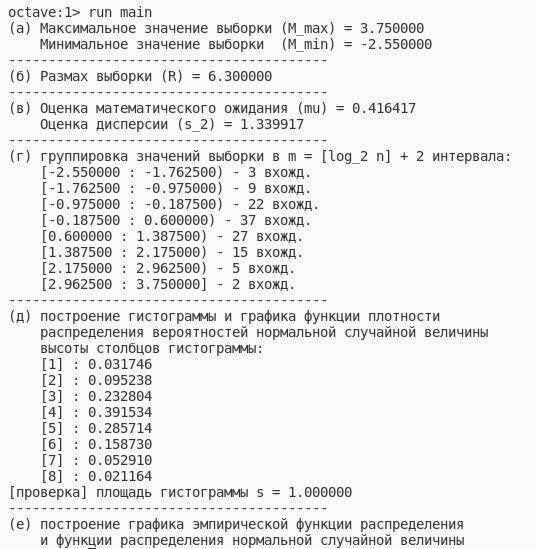
\includegraphics[scale=0.75]{assets/launch.png}
		\caption{Результат работы программы}
	\end{center}
\end{figure}

\begin{figure}[H]
	\begin{center}
		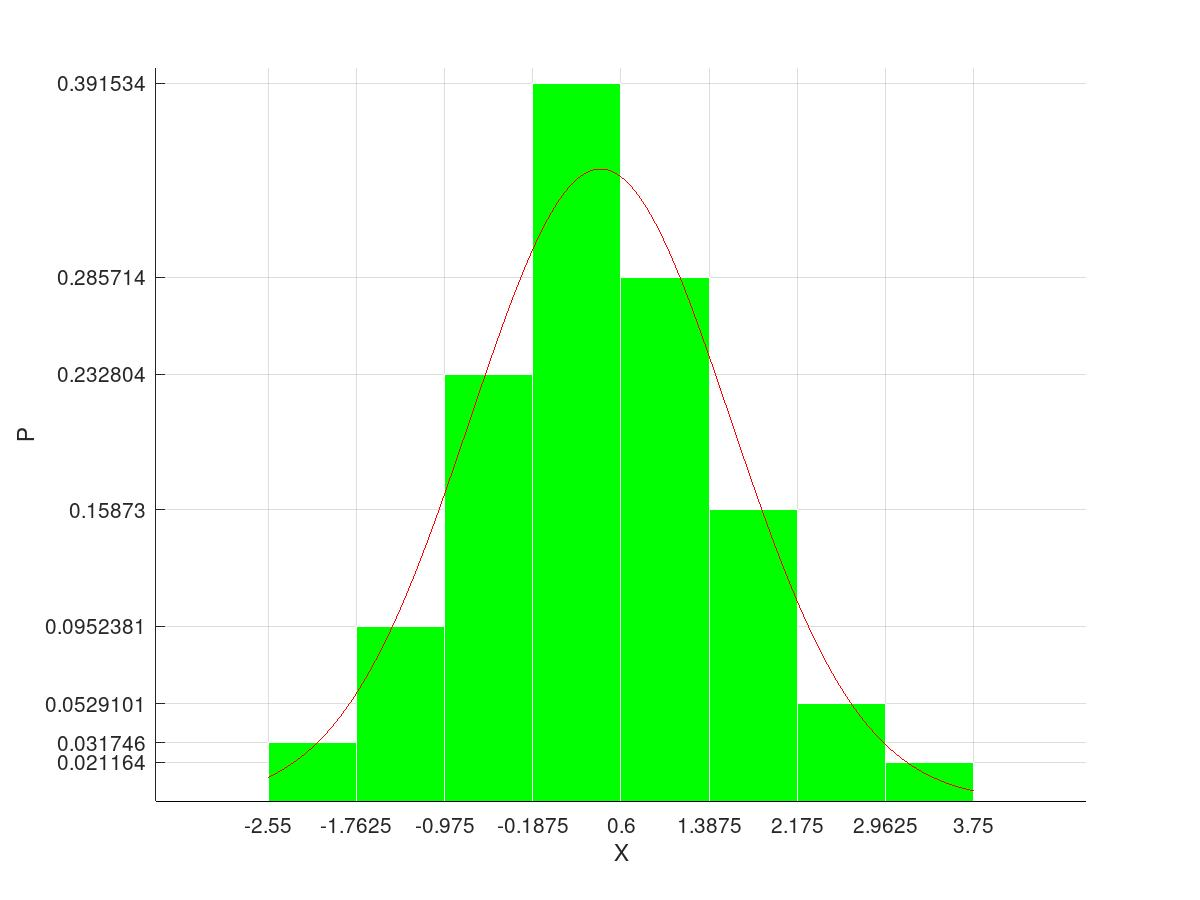
\includegraphics[scale=0.4]{assets/hist.jpg}
		\caption{Гистограмма и график функции плотности распределения вероятностей нормальной случайной величины}
	\end{center}
\end{figure}

\begin{figure}[H]
	\begin{center}
		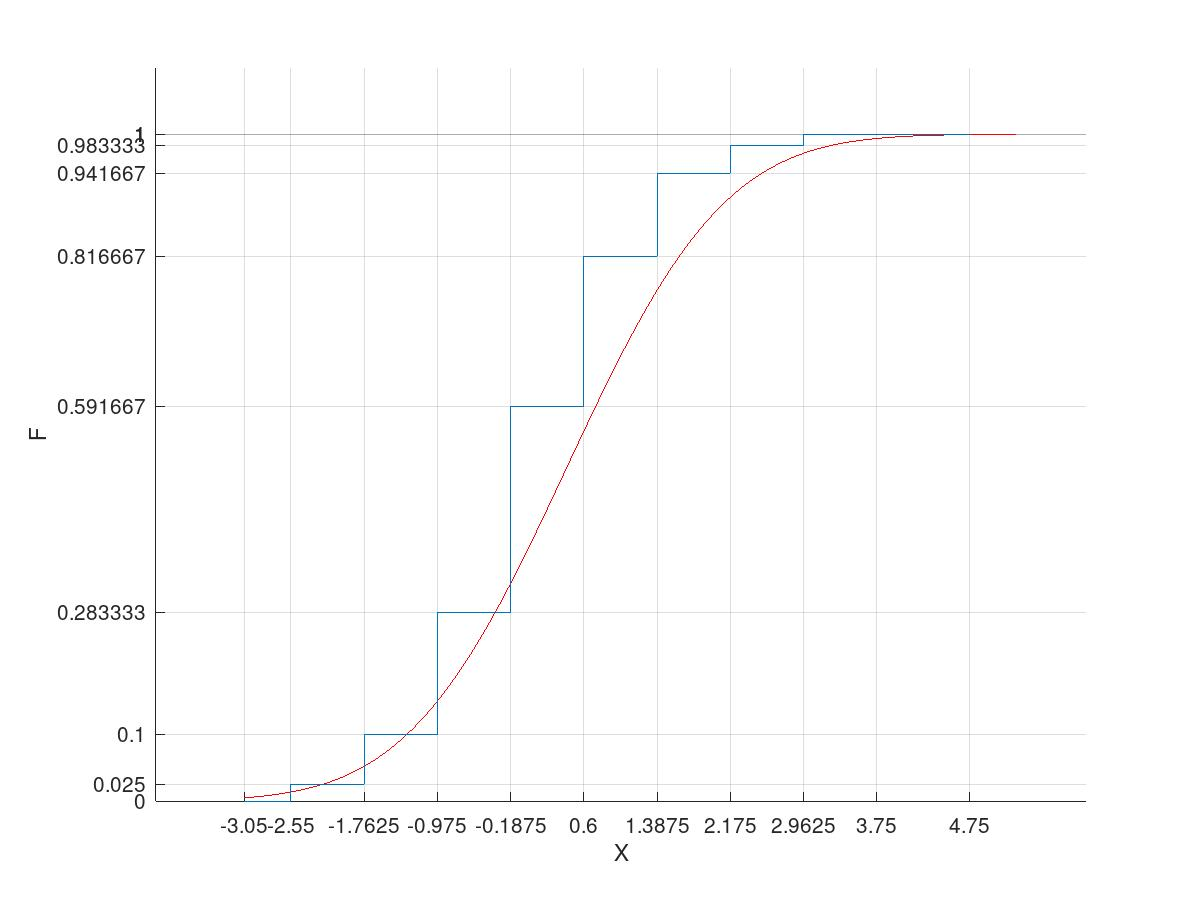
\includegraphics[scale=0.4]{assets/cdf.jpg}
		\caption{График эмпирической функции распределения и функции распределения нормальной случайной величины}
	\end{center}
\end{figure}